\documentclass[10pt,a4paper]{article}
\usepackage[utf8]{inputenc}
\usepackage[T1]{fontenc}
\usepackage[spanish,es-nodecimaldot,es-tabla]{babel}
\usepackage[margin=2.2cm]{geometry}
\usepackage{lmodern,microtype}
\usepackage{mathtools,amssymb,booktabs,array}
\usepackage{graphicx,caption}
\captionsetup{font=small,labelfont=bf,skip=4pt,hypcap=false}
\graphicspath{{03_co2_reformulation_summary_figures/}{03_co2_reformulation_summary_v2_figures/}}
\usepackage{xurl}
\usepackage[hidelinks]{hyperref}
\hypersetup{pdftitle={Reformulación de CO2},pdfsubject={Resumen técnico de cambios, parámetros y resultados}}
\urlstyle{same}
\newcommand{\qb}{q_{\mathrm{bio}}}
\newcommand{\qp}{q_{\mathrm{prod}}}
\newcommand{\qo}{q_{\mathrm{out}}}
\newcommand{\qr}{q_{\mathrm{resp}}}
\newcommand{\qhat}{q_{\mathrm{pred}}}
\newcommand{\ff}{f_{\mathrm{ferm}}}
\newcommand{\clip}{\operatorname{clip}}
\newcommand{\pos}[1]{\left[#1\right]_+}
\newcommand{\code}[1]{\path{#1}}
\setlength{\parskip}{0.25em}
\setlength{\emergencystretch}{2em}
\setlength{\abovedisplayskip}{7pt plus 2pt minus 1pt}
\setlength{\belowdisplayskip}{7pt plus 2pt minus 1pt}
\setlength{\jot}{3pt}
\renewcommand{\arraystretch}{1.08}
\widowpenalty=10000
\clubpenalty=10000

\begin{document}
\begin{center}
{\large\bfseries Reformulación de CO\(_2\)}
\end{center}

\section{Contexto y parámetros comparados}

Se investigó por qué las curvas de CO\(_2\) cambiaban entre el diagnóstico
histórico LAB016--018 y la auditoría LAB019--021. Restaurar solamente el onset
no recuperaba su forma: habían cambiado tanto la cinética como la capa
CO\(_2\). El notebook \code{02_nutrition_structure_comparison} separa estos
efectos cruzando dos theta, dos juegos CO\(_2\) y tres estructuras nutricionales,
sin optimización ni nuevos ajustes.

\code{theta_defaults} es el vector llamado \code{theta_antiguo} en el
notebook 02: once estimaciones naturales y seis defaults. Ambos theta usan
17 parámetros; ninguno falta durante el cálculo. Theta\_full comparte los
once valores y recupera los seis restantes del vector conjunto
\code{theta_multistart_07.csv} de la validación cinética histórica.

Los parámetros \emph{antiguos} son los nueve de la calibración natural
histórica, más el transitorio elegido manualmente para LAB016--018:
$A=0.30$, $\tau_r=4$ h y $\tau_d=12$ h.
Los \emph{nuevos} proceden de dos etapas, manteniendo theta\_full fijo:
\emph{(i)} recalibración de los nueve parámetros CO\(_2\) con
LAB004/005/006/007/008/011, excluyendo LAB010 y reservando LAB012 para
validación interna; \emph{(ii)} ajuste ampliado de
$k_{\mathrm{release}},s_{\mathrm{CO_2}},g_{\mathrm{matrix}},A,\tau_r,\tau_d$
con LAB005/007/008 (peso 1) y LAB019/020/021 (peso 2).
La segunda etapa conserva los seis parámetros de O\(_2\), activación y
rampa de la primera. En la primera etapa se usaron señales CO\(_2\)
corregidas por artefactos de muestreo en LAB004/007/008 y conversión SCCM
corregida. No se reestimó la cinética.

La recalibración sin LAB010, antes del ajuste ampliado, daba
$k_{\mathrm{release}}=0.278349$ h$^{-1}$,
$s_{\mathrm{CO_2}}=2.498908$ y $g_{\mathrm{matrix}}=1.602222$.
Estos tres valores se sustituyeron por los de la columna \emph{Nuevos}
de la tabla 1. El transitorio $A,\tau_r,\tau_d$ se ajustó en la segunda
etapa; no es un resultado de la recalibración sin LAB010.

\begin{center}
\begin{minipage}[t]{0.54\textwidth}
\centering\small
\textbf{Tabla 1. Capa CO\(_2\): juegos congelados.}\par\medskip
\begin{tabular}{@{}lrr@{}}
\toprule Parámetro & Antiguos & Nuevos\\\midrule
$k_{\mathrm{release}}$ [h$^{-1}$] & 0.424588 & 0.096958\\
$s_{\mathrm{CO_2}}$ & 0.351390 & 2.500000\\
$g_{\mathrm{matrix}}$ & 3.115757 & 1.446718\\
$q_{O_2,\max}$ [mg/(g h)] & 0.150000 & 0.253137\\
$\alpha_O$ & 0.195400 & 0.179606\\
$t_{\mathrm{rise}}$ [h] & 64.658704 & 56.741847\\
$g$ & 0.250000 & 0.250011\\
$s$ & 0.735057 & 0.741575\\
$d$ & 1.063910 & 0.457773\\
$A$ & 0.300000 & 1.500000\\
$\tau_r$ [h] & 4.000000 & 0.540335\\
$\tau_d$ [h] & 12.000000 & 4.399251\\
\bottomrule
\end{tabular}
\end{minipage}\hfill
\begin{minipage}[t]{0.43\textwidth}
\centering\small
\textbf{Tabla 2. Diferencias de theta.}\par\medskip
\begin{tabular}{@{}lrr@{}}
\toprule Parámetro & Defaults & Full\\\midrule
$s_N$ & 18.000000 & 8.751446\\
$q_{XG}$ & 0.112500 & 0.081491\\
$q_{XF}$ & 0.112500 & 0.070933\\
$s_G$ & 0.030000 & 0.097455\\
$s_F$ & 0.030000 & 0.178295\\
$m_0$ & 0.010000 & 0.018339\\
\bottomrule
\end{tabular}
\medskip\par\raggedright
Los otros once valores son iguales: $\mu_0$, $q_N$, $\beta_{G0}$,
$\beta_{F0}$, $q_{EG}$, $q_{EF}$, $i_G$, $i_E$, $K_{d0}$,
$\gamma_{G0}$ y $\gamma_{F0}$. Los parámetros de la tabla 1 no pertenecen
a theta.
\end{minipage}
\end{center}

$g$ es el gain nutricional; $g_{\mathrm{matrix}}$ es \code{matrix_gain}.
$s,d$ controlan la activación. $t_{\mathrm{rise}}$ es el tiempo de rampa;
$\tau_r$ es el tiempo de subida del transitorio. Los parámetros sin unidad
indicada en la tabla 1 son adimensionales. El kernel se normaliza por máximo
de grilla en el juego antiguo y por máximo analítico en el nuevo.
$s_N$ se expresa en L (g N)$^{-1}$ h$^{-1}$; $q_{XG},q_{XF},m_0$
en g azúcar (g biomasa)$^{-1}$ h$^{-1}$.

La primera etapa corresponde al notebook
\code{co2_solubility_o2_cross_matrix_2026_full_theta_no_lab010},
resultado natural con theta\_full y capa CO\(_2\) recalibrada.
La segunda se realizó en la auditoría de producción LAB019--021.
Ambos juegos se mantuvieron fijos durante la comparación de estructuras;
onset, condiciones iniciales y dosis son entradas separadas.

\begin{center}\small
\textbf{Tabla 3. Notación de las tasas de CO\(_2\).}\par\medskip
\begin{tabular}{@{}lp{11.0cm}l@{}}
\toprule Símbolo & Significado & Unidad\\\midrule
$q_{\mathrm{bio},0}$ & Producción biológica calculada sin pulsos posteriores de N (con N inicial).
& g CO\(_2\) L$^{-1}$ h$^{-1}$\\
$q_{\mathrm{bio},N}$ & Producción biológica calculada con los pulsos de N.
& g CO\(_2\) L$^{-1}$ h$^{-1}$\\
$\qb$ & Producción biológica efectiva, con rampa, gain y transitorio.
& g CO\(_2\) L$^{-1}$ h$^{-1}$\\
$\qp$ & Producción que entra al depósito disuelto, después de activación y
modulación por O\(_2\).
& g CO\(_2\) L$^{-1}$ h$^{-1}$\\
$\qo$ & Flujo liberado desde el depósito disuelto.
& g CO\(_2\) L$^{-1}$ h$^{-1}$\\
$\qhat$ & Flujo predicho que se compara con el sensor.
& g CO\(_2\) L$^{-1}$ h$^{-1}$\\
$q_{\mathrm{obs}}$ & Flujo observado válido.
& g CO\(_2\) L$^{-1}$ h$^{-1}$\\
\bottomrule
\end{tabular}
\end{center}

\clearpage
\section{Análisis de los resultados del notebook}

La comparación principal usa activación predicha desde la química simulada:
72 curvas, correspondientes a seis LAB, dos theta, dos juegos CO\(_2\) y tres
estructuras. Se añaden 36 diagnósticos de onset manual para LAB016--018,
seis curvas manuales con CO\(_2\) antiguo para LAB019--021 y una figura final
con tres variantes por LAB y theta. Las métricas se toman de las salidas
guardadas en EXECUTED. Se evaluaron RMSE, error de inicio, pico y área, además
de ventanas antes del pulso, 24 h posteriores y cola.

\begin{center}\small
\textbf{Tabla 4. Mediana del RMSE completo por grupo; gate predicho.}\par\medskip
\begin{tabular}{@{}llllrr@{}}
\toprule
Estructura & CO\(_2\) & Theta && LAB016--018 & LAB019--021\\\midrule
Rampa + gain + T & Antiguos & Defaults && 0.2046 & 0.2047\\
Rampa + gain + T & Antiguos & Full && 0.4272 & 0.3245\\
Rampa + gain + T & Nuevos & Defaults && 0.1931 & 0.1391\\
Rampa + gain + T & Nuevos & Full && 0.1094 & 0.1370\\
Directa, sin T & Nuevos & Full && 0.1196 & 0.1400\\
Directa, con T & Nuevos & Full && 0.1282 & 0.1378\\
\bottomrule
\end{tabular}\par\smallskip
Unidades: g CO\(_2\) L$^{-1}$ h$^{-1}$. T denota transitorio. Las opciones
directas omiten rampa y gain; conservan el efecto cinético de N.
\end{center}

Las figuras siguientes adaptan los escenarios del notebook 02 a blanco y negro; las curvas y métricas se verificaron sin reajuste.

\begin{center}
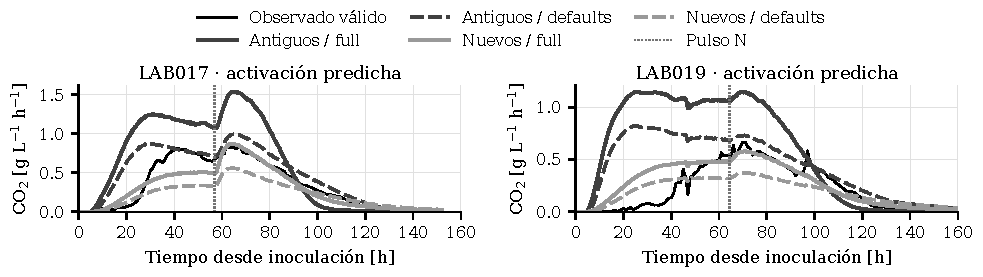
\includegraphics[width=\linewidth]{theta_and_co2_layer.pdf}
\captionof{figure}{Comparación de theta y capa CO\(_2\): LAB017 y LAB019,
ejemplos externo y reciente; activación predicha, rampa/gain/transitorio
conservados. Punteadas: pulsos N. La tabla 4 resume los seis LAB.}
\label{fig:theta-layer}
\end{center}

\paragraph{Efecto de theta.}
Con CO\(_2\) antiguo, theta\_full aumenta los picos y acelera la caída final:
en el diagnóstico manual LAB019--021 los picos pasan de
0.7299/0.5432/0.7128 (theta\_defaults) a 1.1452/0.7845/1.0903 (full).
El cambio tiene una explicación cinética: mayores $s_G,s_F$ reducen
$K_G=\beta_{G0}a_K/s_G$ y $K_F=\beta_{F0}a_K/s_F$, aumentando la actividad
a igual azúcar. La simulación full consume azúcar y produce etanol más rápido,
lo que contribuye a picos altos y menor duración de la cola. También cambian
crecimiento y mantenimiento. El menor RMSE depende de la capa: theta\_defaults
es mejor con parámetros antiguos; full tiene menor RMSE mediano con nuevos.

\paragraph{Efecto de la capa CO\(_2\).}
El juego nuevo combina menor escala de matriz y menor liberación con mayor
solubilidad aparente y un transitorio más intenso y corto. Su cambio conjunto
reduce la sobrepredicción de las configuraciones antiguas y mejora el RMSE
con gate predicho. No se puede atribuir esa mejora a un solo coeficiente.
En la referencia nueva/full, el error mediano de área es $-11.95\%$ en
LAB016--018 y $+2.45\%$ en LAB019--021; con nuevo/theta\_defaults es $-34.38\%$
y $-26.24\%$, respectivamente.

\paragraph{Rampa, transitorio e inicio.}
Retirar rampa/gain sin reajuste no mejora uniformemente la comparación.
Con antiguo/full, el RMSE mediano reciente pasa de 0.3245 a 0.5083
(directa) y 0.5319 (directa con T). Con nuevo/full las diferencias globales
son menores, aunque cambian las ventanas y el área; agregar T a la opción
directa no asegura un mejor RMSE. Con gate predicho, el inicio reciente se
anticipa 13--21 h con antiguo/full y 5--16 h con nuevo/full. El onset manual
reduce ese desfase; no corrige por sí solo amplitud, química ni cola.

\paragraph{Química y alcance de la evaluación.}
Las trayectorias full agotan antes G+F; en LAB019--020 anticipan parte de su
consumo y sobrepredicen etanol en tiempos intermedios. Ambos theta consumen
N inicial demasiado pronto respecto de las mediciones. Un buen ajuste de
CO\(_2\) no valida por sí solo la química. LAB019--021 participaron en la
calibración del juego nuevo; LAB016--018 ya habían sido explorados y usan
condiciones iniciales proxy y dosis supuestas. No son holdouts nuevos y
estrictos. Las figuras manuales son diagnósticos condicionados al inicio.

\begin{center}
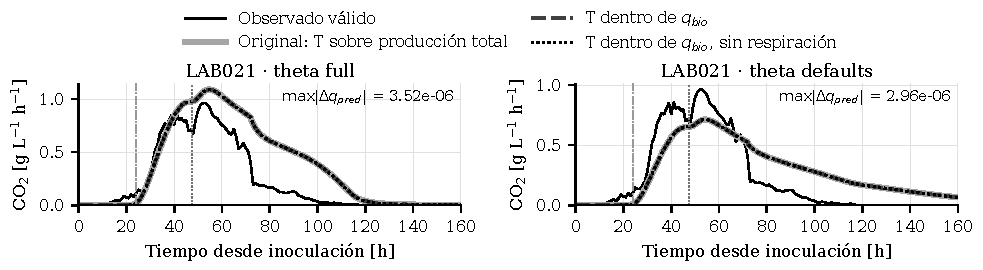
\includegraphics[width=\linewidth]{transient_and_respiration.pdf}
\captionof{figure}{LAB021: tres variantes, parámetros antiguos y ambos
theta. Se indica $\max|\Delta q_{\mathrm{pred}}|$ al retirar respiración
[g L$^{-1}$ h$^{-1}$]. Pulso: 47.5 h (punteada); onset manual: 24 h
(trazo y punto). La superposición no implica buen ajuste al observado.}
\label{fig:transient}
\end{center}

\clearpage
\section{Cambio de ecuación y significado de la nutrición}

Defínase únicamente como abreviatura de rampa y gain
\begin{equation}
\mathcal R(t)=\Bigl[[1+(g-1)r(t)]q_{\mathrm{bio},0}(t)
+r(t)\bigl(q_{\mathrm{bio},N}(t)-q_{\mathrm{bio},0}(t)\bigr)\Bigr]_+,
\label{eq:R}
\end{equation}
con $[v]_+=\max(v,0)$ y
$r=\clip((t-t_p)/t_{\mathrm{rise}},0,1)$, anclada al primer pulso;
si no hay nutrición, $r=0$. La formulación anterior era
% La mezcla conserva el gain histórico; no es una interpolación convexa.
\begin{equation}
\qp^{\mathrm{original}}=a(1+T_N)(\ff\mathcal R+\qr).
\label{eq:original}
\end{equation}
El transitorio actuaba sobre fermentación y respiración. Se compararon los
siguientes cambios manteniendo las mismas entradas y reintegrando el depósito:
\begin{center}\small
\begin{tabular}{@{}lp{10.0cm}@{}}
\toprule Variante & Producción que ingresa al depósito\\\midrule
Original & $a(1+T_N)(\ff\mathcal R+\qr)$\\
Transitorio dentro de $\qb$ & $a[\ff(1+T_N)\mathcal R+\qr]$\\
Además, sin respiración & $a\ff(1+T_N)\mathcal R$\\
\bottomrule
\end{tabular}
\end{center}
La variante conservada define
\begin{equation}
\boxed{\qb=(1+T_N)\mathcal R,\qquad \qp=a\ff\qb.}
\label{eq:final}
\end{equation}
Así, $\qb$ incluye rampa, gain y transitorio, antes de O\(_2\) y activación.
Con $r=1$, $\mathcal R=[q_{\mathrm{bio},N}+(g-1)q_{\mathrm{bio},0}]_+$:
el gain no multiplica por sí solo toda la trayectoria con N.
Se retira el aporte aditivo respiratorio, no el oxígeno. Se conservan la
cinética, $r,g$, activación, modulación fermentativa, depósito, liberación y
escala de matriz. Mover T retira $aT_N\qr$; omitir además respiración retira
de la referencia $a(1+T_N)\qr$. La parte fermentativa es algebraicamente igual.

En la figura final LAB019--021, con CO\(_2\) antiguo, onset 28/32/24 h y
ambos theta, mover T cambia $\qhat$ hasta $6.7\times10^{-16}$ g/L/h;
omitir respiración cambia hasta $3.52\times10^{-6}$ g/L/h, menos de
0.00042\% del pico de cada curva. La superposición fue verificada y no
corresponde a reutilizar una misma curva. Es evidencia para estos casos,
no equivalencia universal si el aporte respiratorio es significativo.
La figura~\ref{fig:transient} muestra LAB021, que presenta la mayor
diferencia absoluta entre variantes en este conjunto.

\subsection*{Transitorio y dosis de referencia}
\begin{align}
T_N(t)&=A\sum_j\frac{\Delta N_j}{N_{\mathrm{ref}}}K_j(t),&
N_{\mathrm{ref}}&=0.14\ \mathrm{g\,N\,L^{-1}},\label{eq:T}\\
K_j(t)&=\frac{(1-e^{-u_j/\tau_r})e^{-u_j/\tau_d}}{\mathcal N_j},&
u_j&=\max(t-t_j,0).\label{eq:kernel}
\end{align}
$T_N$ es un incremento adimensional que sube y decae; $1+T_N$ es su
multiplicador. $A$ fija amplitud por dosis de referencia y $\tau_r,\tau_d$
sus tiempos. $\mathcal N_j$ es el máximo en la grilla antigua o el máximo
analítico nuevo, alcanzado en $u^*=\tau_r\ln(1+\tau_d/\tau_r)$.
Se conserva $N_{\mathrm{ref}}$: proviene del protocolo asumido LAB016--018,
$(1.0+0.4)$ g de productos en 2 L y conversión de 0.20 g N/g producto,
que da $(1.4)(0.20)/2=0.14$ g N/L. No es una medición de YAN ni una escala
fisiológica. Otra dosis cambia $\Delta N_j$, manteniendo $N_{\mathrm{ref}}$;
la proporcionalidad lineal es un supuesto, no una validación para toda dosis.
Por ejemplo, los pulsos de 0.08 g N/L de LAB019--021 usan el cociente
$0.08/0.14$, no una nueva referencia.

\subsection*{Por qué aparecen $T_N$ y $q_{\mathrm{bio},N}$}
$q_{\mathrm{bio},N}$ es una tasa CO\(_2\) calculada desde los estados de la
simulación con pulsos de N. $T_N$ es una corrección transitoria adicional de
actividad; no es otra tasa ni otro salto de N. No modifica nuevamente
$X,G,F,E$ en la cinética. Se representan dos mecanismos de la misma adición:
cambio de estados y reactivación efectiva. Pueden solaparse si la cinética ya
explica esa reactivación. Agruparlos en $\qb$ no elimina esa posible
redundancia ni prueba su identificabilidad independiente.

\clearpage
\section{Expresión química de la producción biológica}

Para $k\in\{0,N\}$,
\begin{equation}
q_{\mathrm{bio},k}=Y_{\mathrm{CO_2/E}}X_k
\left(\beta_{G0}\varphi_{G,k}+\beta_{F0}\varphi_{F,k}\right),
\label{eq:raw}
\end{equation}
\begin{align}
\varphi_{G,k}&=a_\beta(T)\frac{G_k}{G_k+K_G(T)}
\frac{1}{1+i_E(T)E_k},\label{eq:phiG}\\
\varphi_{F,k}&=a_\beta(T)\frac{F_k}{F_k+K_F(T)}
\frac{1}{1+i_G(T)G_k}\frac{1}{1+i_E(T)E_k}.\label{eq:phiF}
\end{align}
$X$ es biomasa viable; $G,F,E,N$ son glucosa, fructosa, etanol y N asimilable,
en g/L (equivalentes a kg/m$^3$ del código). Las fracciones de azúcar son
saturaciones; E inhibe ambas contribuciones y G inhibe adicionalmente
fructosa. El subíndice 0 significa \emph{sin pulsos posteriores de N}, no
tiempo inicial ni N inicial nulo. Ambas trayectorias comparten theta,
temperatura y condiciones iniciales.

Con $T_K=T+273.15$ y $R=8.314$ J mol$^{-1}$ K$^{-1}$,
\begin{align}
a_\beta&=\exp\!\left[\frac{11000(T_K-296.15)}{296.15RT_K}\right],&
a_K&=\exp\!\left[\frac{46055(T_K-293.15)}{293.15RT_K}\right],\label{eq:thermal}\\
K_G&=\frac{\beta_{G0}}{s_G}a_K,&K_F&=\frac{\beta_{F0}}{s_F}a_K,\label{eq:K}\\
i_G(T)&=i_G/a_K,&i_E(T)&=i_E/a_K.\label{eq:i}
\end{align}
$K_G,K_F$ son concentraciones; $i_G,i_E$ tienen unidades de concentración
inversa. Los $\beta$ son tasas de etanol por biomasa y hora; $s_G,s_F$ son
esas tasas divididas por concentración de azúcar. Las constantes térmicas
son comunes a ambos theta.

El coeficiente conservado del código es
$Y_{\mathrm{CO_2/E}}=44.01/[2(46.07)]=0.4776427$ g CO\(_2\)/g E.
Es la mitad del cociente ideal CO\(_2\)/etanol $44.01/46.07$; no se corrige
en esta comparación. Se distingue del rendimiento CO\(_2\)/azúcar y de la
conversión SCCM del sensor.

El N afecta los estados mediante
\begin{align}
\psi_k&=a_\mu\frac{N_k}{N_k+K_N},&
a_\mu&=\exp\!\left[\frac{59453(T_K-300)}{300RT_K}\right],&
K_N&=\frac{\mu_0}{s_N}a_K,\label{eq:mu}\\
\dot X_k&=(\mu_0\psi_k-k_{d,k})X_k,&
\dot N_k&=-q_N\psi_kX_k,\label{eq:XN}
\end{align}
con saltos $N_N(t_j^+)=N_N(t_j^-)+\Delta N_j$. El consumo y la producción
cinéticos se calculan como
\begin{align}
\dot G_k&=-X_k\left[q_{XG}\psi_k+q_{EG}\varphi_{G,k}
+m(T)\chi_k\frac{G_k}{G_k+F_k}\right],\label{eq:G}\\
\dot F_k&=-X_k\left[q_{XF}\psi_k+q_{EF}\varphi_{F,k}
+m(T)\chi_k\frac{F_k}{G_k+F_k}\right],\label{eq:F}\\
\dot E_k&=X_k(\beta_{G0}\varphi_{G,k}+\beta_{F0}\varphi_{F,k}),\label{eq:E}\\
m(T)&=m_0\exp\!\left[\frac{37681(T_K-293.3)}{293.3RT_K}\right],&
\chi_k&=\frac{G_k+F_k}{G_k+F_k+1}.\label{eq:maintenance}
\end{align}
El 1 de $\chi_k$ representa 1 g/L de azúcar. $q_N$ es consumo específico de N,
no producción de CO\(_2\). La muerte celular conserva
\begin{align}
T_d(E_k)&=-0.0001E_k^3+0.0049E_k^2-0.1279E_k+315.89,\label{eq:Td}\\
k_{d,k}&=\begin{cases}
0,&T_K<T_d(E_k),\\
K_{d0}\exp\!\left[0.0415E_k+
\dfrac{130000(T_K-305.65)}{305.65RT_K}\right],&T_K\ge T_d(E_k).
\end{cases}\label{eq:kd}
\end{align}
$T_d$ está en K y $k_d$ en h$^{-1}$; E se introduce en g/L.
Los $q_{XG},q_{XF}$ ponderan consumo asociado al crecimiento;
$q_{EG},q_{EF}$ ponderan el fermentativo y $m$ el mantenimiento.
La capa CO\(_2\) se aplica después y no retroalimenta estos balances.
Las formas de G/F, inhibición, crecimiento y temperatura se relacionan
directamente con Zenteno et al.~\cite{zenteno}; la ecuación nutricional
completa es una adaptación, no una reproducción literal de ese modelo.

\clearpage
\section{Oxígeno, activación, emisión y límites de interpretación}

El factor fermentativo y el O\(_2\) conservados son
\begin{align}
\ff&=0.08+0.92\frac{0.75^2}{0.75^2+O^2},&
\dot O&=-q_{O_2,\max}X_{\mathrm{eff}}\frac{O}{0.25+O},\label{eq:O}\\
X_{\mathrm{eff}}&=\pos{X_0+r(X_N-X_0)},&
O(0)&=\alpha_O O_{\mathrm{sat}}(0),\label{eq:Xeff}\\
O_{\mathrm{sat}}&=8.6e^{-0.024(T-20)}e^{-0.002E_N}e^{-0.001(G_N+F_N)}.
\label{eq:Osat}
\end{align}
$O,O_{\mathrm{sat}}$ están en mg O\(_2\)/L; 0.25 y 0.75 tienen las mismas
unidades. No hay reposición de O\(_2\); gain y transitorio no multiplican
$X_{\mathrm{eff}}$. El aporte retirado era
$\qr=(44.01/32000)q_{O_2,\max}X_{\mathrm{eff}}O/(0.25+O)$.

La activación se expresa como
\begin{equation}
a=3z^2-2z^3,\qquad
z=\clip\left(\frac{t-[L+s(U-L)]}{\max(d(U-L),0.25)},0,1\right).
\label{eq:gate}
\end{equation}
En el notebook 02, $[L,U]$ se obtiene del primer descenso simulado de G+F de
5 g/L o aumento de E de 2 g/L, y su punto anterior. En modo manual,
$[L,U]=[0,t_{\mathrm{onset}}]$. El piso de duración es 0.25 h; si $L=U$ se
usa un escalón. Por ello onset no es un desplazamiento directo de toda la curva.
La auditoría térmica posterior utiliza, sólo en ese notebook,
\textbf{6 g/L de G+F consumidos o 2 g/L de etanol generado}, ambos respecto
del inicio simulado. La condición es ``o'', no ``y''; el cambio no modifica
las métricas históricas del notebook 02 presentadas antes.
Con un intervalo de grilla de 0.25 h y las fracciones antiguas, la transición
suave dura aproximadamente 0.266 h (16 min), no una latencia de varias horas.

El depósito y el flujo comparado con el sensor son
\begin{align}
\dot C&=\qp-\qo,\quad C(0)=0,&
\qo&=k_{\mathrm{release}}C\left(0.05+0.95\frac{C}{C+C_{\mathrm{sat}}}\right),\label{eq:pool}\\
C_{\mathrm{sat}}&=s_{\mathrm{CO_2}}1.69e^{-0.032(T-20)}e^{0.0016E_N}
e^{-0.0012(G_N+F_N)},&
\qhat&=g_{\mathrm{matrix}}\qo.\label{eq:sensor}
\end{align}
$C,C_{\mathrm{sat}}$ se expresan en g CO\(_2\)/L; todas las tasas $q$ de
CO\(_2\) en g L$^{-1}$ h$^{-1}$ y $t$ en h. Las correlaciones usan $T$ en
grados Celsius y $E,G,F$ en g/L. El depósito se integra con Euler a 0.25 h,
limitando la salida por el CO\(_2\) disponible. $C_{\mathrm{sat}}$ modula
liberación, no impone una cota rígida de concentración. La distinción entre
producción y emisión tiene antecedente en Zenteno et al.~\cite{zenteno};
la ley racional continua presente es un cierre propio.

La observación emplea \code{SCCM_CORRECTED}, después de corrección del cero,
recorte a no negativos y mediana horaria. Para volumen fijo de 2 L,
\begin{equation}
q_{\mathrm{obs}}=Q_{\mathrm{corr,SCCM}}
\frac{44.0095\,(60)\,(0.74)}{1000\,(24.16)\,(2.0)}
=0.04043919288\,Q_{\mathrm{corr,SCCM}}.
\label{eq:sccm}
\end{equation}
Esta conversión es común a las configuraciones; no cambia al seleccionar
theta\_defaults o parámetros antiguos. Tampoco es $Y_{\mathrm{CO_2/E}}$
ni $g_{\mathrm{matrix}}$.

La reactivación por N con poco crecimiento tiene respaldo en
Malherbe et al.~\cite{malherbe}, David et al.~\cite{david} y
Seguinot et al.~\cite{seguinot}. David distribuye N durante un intervalo de
utilización: inspira la rampa, pero no nuestra mezcla contrafactual.
El kernel exacto, su referencia de dosis, el gain, la activación y las
correlaciones efectivas no se verificaron como tales en los papers revisados.
La reformulación organiza mecanismos conservados y omite un aporte pequeño
en los casos evaluados; no resuelve por sí sola el inicio, los desajustes
químicos ni la posible superposición entre efecto cinético y transitorio.
Las secciones anteriores describen el notebook 02; la sección siguiente incorpora
la auditoría térmica posterior, distinguiendo su criterio de activación y sus ajustes.


\clearpage
\section{Temperatura: evidencia y limitaciones del modelo}

\paragraph{Qué queremos representar.}
El objetivo es que una misma parametrización describa fermentaciones con
temperatura constante y con perfiles variables, usando $T(t)$ como entrada.
La temperatura modifica crecimiento, fermentación, mantenimiento,
saturaciones e inhibiciones. Estos efectos se combinan: un cambio térmico no
se traduce en un único multiplicador del CO$_2$. Las constantes térmicas son
comunes a ambos theta, pero sus diferencias de saturación y consumo cambian
la respuesta efectiva y el avance de la fermentación.
Además, $q_{\mathrm{prod}}$ entra al depósito disuelto y $q_{\mathrm{out}}$
sale de él: la emisión medida puede responder con demora y distinta
magnitud respecto de la producción biológica.

\paragraph{Qué se probó.}
La auditoría \code{lab019_021_co2_temperature_shape_audit} usa la ecuación
simplificada sin aporte respiratorio, la capa CO$_2$ antigua y ambos theta
congelados. Su activación utiliza \textbf{6 g/L de G+F consumidos o 2 g/L de
etanol generado}, respecto del inicio simulado. Se exploran un reloj posterior
sobre la producción basal, una adaptación inicial, una liberación $k(T)$ y
un reloj aplicado a toda la cinética. El reloj posterior conserva la química;
el cinético reconstruye los estados. Son hipótesis diagnósticas añadidas a
la temperatura ya presente, no una recalibración de theta.

Los parámetros añadidos se ajustan con LAB005/007/008 (peso 1) y
LAB019/020/021 (peso 2); LAB011/012 seleccionan candidatos y LAB016/017/018
aportan evaluación externa. LAB010 sólo se usa como sensibilidad.
La nueva auditoría tiene ajustes térmicos; la comparación del notebook 02
sigue siendo una comparación de estructuras sin reajuste.

\paragraph{Qué muestran los cambios de temperatura.}
\begin{center}\small
\textbf{Tabla 5. Cambio relativo de CO$_2$ en ventanas de cambio térmico.}\par\medskip
\begin{tabular}{@{}lrrrrrr@{}}
\toprule
& $\Delta T$ & Observado & \multicolumn{2}{c}{Referencia} & \multicolumn{2}{c}{Cinético seleccionado}\\
LAB & [$^\circ$C] & [\%] & Full [\%] & Defaults [\%] & Full [\%] & Defaults [\%]\\\midrule
019 & $+2.8$ & $+16.8$ & $-33.0$ & $-9.9$ & $+38.7$ & $+18.5$\\
020 & $+2.0$ & $+20.6$ & $-10.3$ & $-6.3$ & $+24.7$ & $+12.4$\\
021 & $-3.0$ & $-64.9$ & $-22.2$ & $-19.2$ & $-38.2$ & $-34.5$\\
\bottomrule
\end{tabular}\par\smallskip
Cambio $100(q_{\text{después}}/q_{\text{antes}}-1)$ entre medianas de
CO$_2$: 3--1 h antes y 3--5 h después del cambio de setpoint, con tres puntos
horarios válidos por ventana. Se usa $\Delta T$ medida, no sólo el setpoint.
\end{center}
La referencia predice una disminución donde LAB019 y LAB020 muestran un
aumento. El reloj cinético recupera ese aumento, pero no su magnitud de forma
uniforme. En LAB021 sigue subestimando la caída relativa.
La figura~\ref{fig:thermal-co2} compara las trayectorias completas.
Estas ventanas incluyen progreso fermentativo y memoria del depósito;
aunque no contienen un pulso N próximo, no aíslan causalmente la temperatura.

\paragraph{Qué sigue sin resolverse.}
Mejorar el error global de CO$_2$ no asegura reproducir los cambios locales
ni validar biomasa, N, azúcar y etanol. En LAB021/full, el candidato cinético
reduce el RMSE de G+F de 9.90 a 4.49 g/L, pero aumenta el de etanol de 3.57 a
5.86 g/L y el de biomasa viable de 0.619 a 0.637 g/L.
La adaptación posterior full alcanza el límite de 60 h y su reloj cinético
elige 12000 K, máximo probado: no son parámetros fisiológicos identificados.
La adaptación ensayada describe el arranque, no una readaptación tras cada
cambio térmico. La prueba de temperatura constante cambia sólo el reloj
posterior y $k(T)$; no es una simulación completamente isotérmica.
La aparente preferencia de defaults por temperatura constante y de full por
perfiles variables sigue siendo una hipótesis: aún falta evaluar los lotes
separados por ese criterio y buscar una parametrización común consistente
con CO$_2$ y química. Los lotes externos ya fueron explorados y conservan
supuestos de ICs y dosis; no constituyen una validación independiente nueva.

\clearpage
\begin{center}
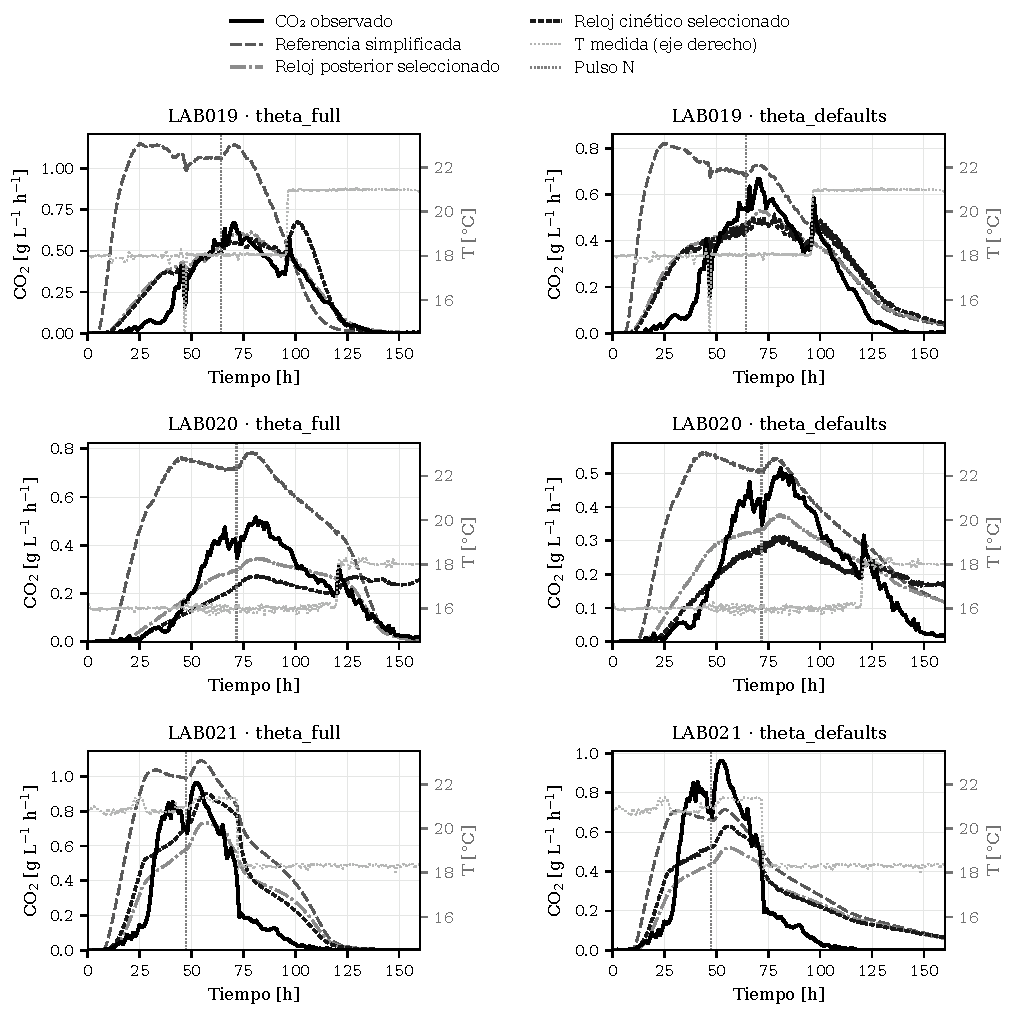
\includegraphics[width=\linewidth]{thermal_co2_comparison.pdf}
\captionof{figure}{LAB019--021: CO$_2$ observado, referencia simplificada,
reloj posterior seleccionado y reloj cinético seleccionado para ambos theta.
La temperatura medida se muestra en el eje derecho; su suavizado es sólo
visual. Las líneas verticales indican pulsos N. Se conserva la capa CO$_2$
antigua y la activación de 6 g/L de G+F o 2 g/L de etanol. Comparaciones
reproducidas del notebook térmico sin nuevos ajustes.}
\label{fig:thermal-co2}
\end{center}
La comparación distingue el ajuste de la forma global de la respuesta local:
el candidato posterior puede mejorar la curva completa sin recuperar el
sentido de los aumentos de CO$_2$ de LAB019 y LAB020. Los relojes cinéticos
mejoran parte de esa respuesta, pero no explican completamente LAB021.

\clearpage
\begin{center}
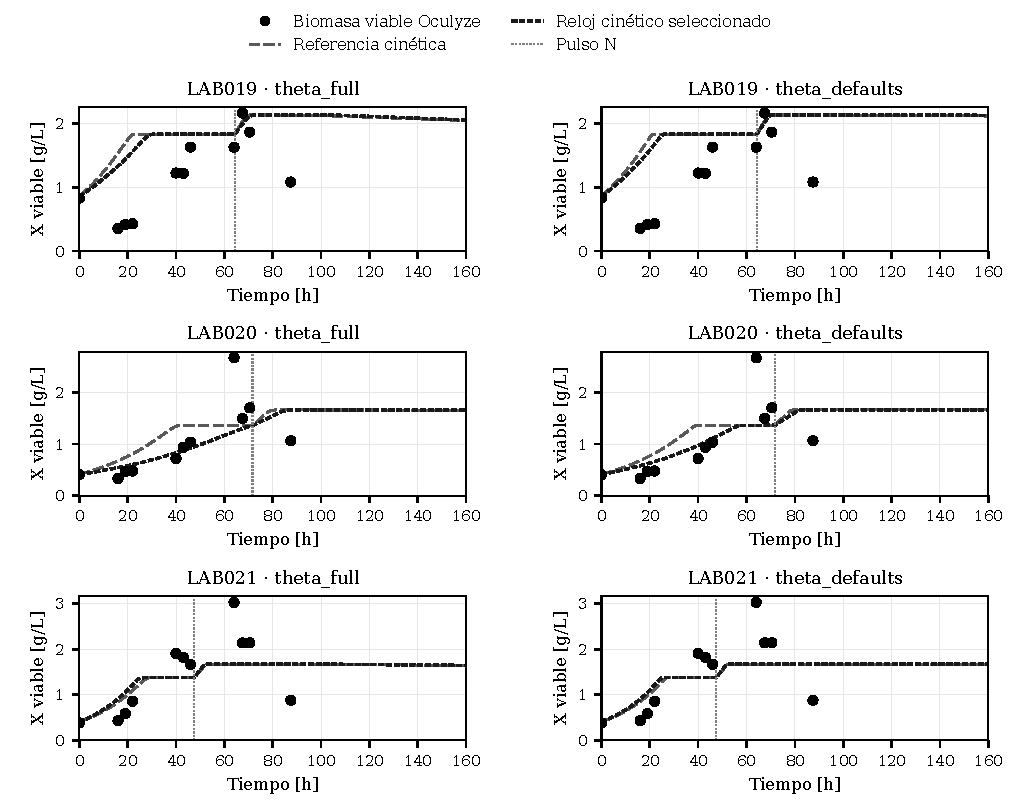
\includegraphics[width=\linewidth]{thermal_biomass_comparison.pdf}
\captionof{figure}{Biomasa viable de LAB019--021: referencia cinética y reloj
cinético seleccionado, frente a las 33 mediciones Oculyze (11 por lote), para
ambos theta. Son los perfiles de la comparación de estados del notebook,
reproducidos sin reajuste. La biomasa observada se obtiene de concentración
celular $\times$ 0.03 $\times$ viabilidad/100 en g/L; se usa tiempo de muestreo,
m1 en $t=0$ y concentración cruda sin restar CERO, conservando las ICs.
Las líneas verticales indican pulsos N.}
\label{fig:thermal-biomass}
\end{center}
Las mediciones permiten contrastar la cinética, además del CO$_2$.
Los relojes desplazan el crecimiento, pero no reproducen uniformemente
los máximos y descensos observados. Las métricas de biomasa excluyen m1;
las mediciones no se usaron para ajustar los parámetros térmicos.
Por ello, un mejor ajuste de emisión debe comprobarse también contra
los estados internos antes de interpretar la corrección como mecanismo.

\begin{thebibliography}{4}
\small\setlength{\itemsep}{0.1em}\setlength{\parskip}{0pt}
\bibitem{zenteno} Zenteno, M.~I., Pérez-Correa, J.~R., Gelmi, C.~A., y Agosin, E.
(2010). Modeling temperature gradients in wine fermentation tanks.
\emph{Journal of Food Engineering}, 99, 40--48. doi:10.1016/j.jfoodeng.2010.01.033.
\bibitem{malherbe} Malherbe, S., Fromion, V., Hilgert, N., y Sablayrolles, J.-M.
(2004). Modeling the effects of assimilable nitrogen and temperature on
fermentation kinetics in enological conditions.
\emph{Biotechnology and Bioengineering}, 86, 261--272. doi:10.1002/bit.20075.
\bibitem{david} David, R., Dochain, D., Mouret, J.-R., Vande Wouwer, A., y
Sablayrolles, J.-M. (2012). Modeling of the boost effect originated by nitrogen
addition during wine-making fermentation. \emph{MED 2012}, 353--358. IEEE.
\bibitem{seguinot} Seguinot, P., et al. (2018). Impact of the timing and the nature
of nitrogen additions on the production kinetics of fermentative aromas by
\emph{Saccharomyces cerevisiae} during winemaking fermentation in synthetic
media. \emph{Food Microbiology}, 76, 29--39. doi:10.1016/j.fm.2018.04.005.
\end{thebibliography}
\end{document}
